\documentclass[a4paper, 10pt]{article}
%\usepackage{fontspec}
%\setmainfont{Lato}
\usepackage{pgf}
\usepackage{eurosym}
\usepackage{graphicx}
\usepackage{wasysym}
\usepackage{hyperref}
\usepackage{listings}
\usepackage{pxfonts}
\usepackage{verbatim}
\usepackage{color}
\usepackage{xcolor}
\usepackage{wrapfig}
\usepackage{enumitem}
\usepackage{booktabs}
\usepackage{gensymb}
\usepackage{tabularx}
\usepackage{currfile}

\hypersetup{
    bookmarks=true,         % show bookmarks bar?
    unicode=true,          % non-Latin characters in Acrobat’s bookmarks
    pdftoolbar=true,        % show Acrobat’s toolbar?
    pdfmenubar=true,        % show Acrobat’s menu?
    pdffitwindow=true,     % window fit to page when opened
    pdftitle={Assessments},    % title
    pdfauthor={Paul Vesey},     % author
    pdfsubject={Advanced Graphics Assignment },   % subject of the document
    pdfcreator={},   % creator of the document
    pdfproducer={xelatex}, % producer of the document
    pdfkeywords={'Graphics' }, % list of keywords
    pdfnewwindow=true,      % links in new PDF window
    colorlinks=true,       % false: boxed links; true: colored links
    linkcolor=violet,          % color of internal links (change box color with linkbordercolor)
    citecolor=magenta,        % color of links to bibliography
    filecolor=red,      % color of file links
    urlcolor=blue           % color of external links
}

\setlength\parindent{0pt}
\begin{document}

\lstset{language=HTML,
				basicstyle=\small,
				breaklines=true,
        numbers=left,
        numberstyle=\tiny,
        showstringspaces=false,
        aboveskip=-20pt,
        frame=leftline
        }
				
\begin{table}%
	\begin{minipage}{0.4\textwidth}%
			
\includegraphics[width=1\textwidth]{./img/LITlogo.jpg}
	\end{minipage}
	\qquad
	\centering
	\parbox{0.4\textwidth}{
		\begin{large}			
			\begin{tabular}{| r | l |} \hline
				Subject: & \textbf{Advanced Graphics}\\
								 & \textbf{\& Visualisation}\\
				Course: & \textbf{Interior Design Y3}\\
				Session: & \textbf{Autumn 2020}\\
				Lecturer: & \textbf{Paul Vesey \footnotesize{BEng, MIE, HDip}}\\
				Filename: & \footnotesize{\currfilename}\\
				\hline
			\end{tabular}
		\end{large}			
	}
\end{table}
\vspace{0.25cm}	
	
\part*{Assignment 1 – Pallasgreen Community Centre with  Revit \& V-Ray }

\begin{tabularx}{\textwidth}{ |X|X| }
	\hline
	\textbf{Issue Date:} & 5$^{th}$ November 2020 \\
	\hline 
	\textbf{Submission Date:}  & 7$^{th}$ December 2020  \\
	\hline
\end{tabularx}


\section*{Continuous Assessment Marks}
This assignment will account for 30\% of the 100\% allocated for continuous assessment in this module

\section*{Assignment Outline}
In this assignment you will create a number of drawings and 3 high quality V-Ray renders from the Revit model of the Pallasgreen Community Centre for Studio Project 1.  The original model is based on the Autocad drawings provided by the client.  The output from this project can be used within your Design Studio Submission\\

You are to create the following, as per the Design Studio spec:

\begin{enumerate}
	\item Plans, Elevations and Sections to scale
	\item 3D Views
	\item V-Ray Renders (3) of your design
	\item Documentation of your render production process.
\end{enumerate}

We will be working through the production processes of this work over the course of the semester.\\

You have free reign to edit the materials used in the model as you see fit.\\


\newpage

\section*{Production Method}

You should make full use of the tools available to you for the production of these images.  These include the suite of tools available within Revit and V-Ray for materials, lighting, HDR, Image channels, and post production within Photoshop.\\

As part of this assignment you are required to submit a two page report on the production methodology used for your images.  This report should include details of the functionality used, exposure values, intensity values, atmospheric or any other effects used in V-Ray.  It should also detail the usage of Photoshop for compositing and any other modifications made. \\

A suggested approach/methodology is provided below:

\begin{itemize}
	\item Choose the best 3 of your 10 camera angles and positions
	\item Lock the view and orientation of these 3 images to ensure that no framing errors are introduced
	\item Determine the best exposure values for each image by rendering in V-Ray's draft quality.	
	\item Using the V-Ray Appearance and Asset Manager tools, override the Revit Materials with appropriate V-Ray materials.
	\item Set the Resolution of your images to 1920 x 1080.  Also ensure that you have selected appropriate render channels with V-Ray to aid post production in Photoshop.
	\item Consider using the V-Ray lens effects settings to add Bloom/Glare, and lens scratches to make the images more realistic
	\item Create 5 bracketed images of each render scene that can be used later in Photoshop to create HDR images.
	\item In either Photoshop or the V-Ray frame buffer, LUTs is to be applied for color correction or artistic color manipulation. 
\end{itemize}


\section*{File formats and specifications}

\begin{tabularx}{\textwidth}{ |X|X|X| }
	\hline
	\textbf{File Type:} & file extension & additional information\\
	\hline 
	Revit Model  & .rvt & Revit 2021 \\
	Plans & .pdf & LIT A1 Sheets \\
	Elevations & .pdf & LIT A1 Sheets \\
	Sections & .pdf & LIT A1 Sheets \\
	Photoshop  & .psd &  \\	
	Renders  & .png & 1920 x 1080 px\\
	\hline
\end{tabularx}




\section*{Submission}
Upon completion, create a single zip file of your Revit model, drawings, render output, and methodology report.  The files should be placed in a logical folder structure reflective of the file content and the production method.  You should also have one folder titled 'FinalRenders' where duplicates of your final images are placed.  Upload this single zip file to MS Teams on or before the submission deadline.


\begin{figure}[h]
	\centering
	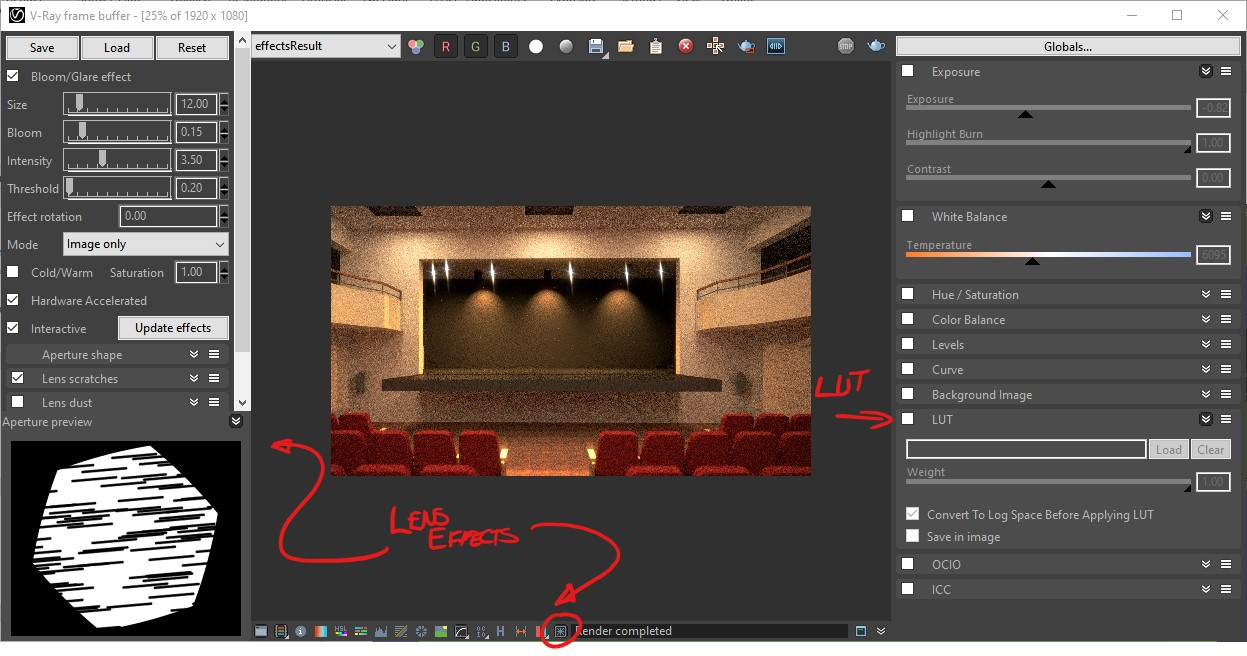
\includegraphics[width=1.0\linewidth]{./img/VRayFrameBuffer.jpg}
	\caption{V-Ray Frame Buffer}
	\label{fig:VRayFrameBuffer}
\end{figure}

\begin{figure}[h]
	\centering
	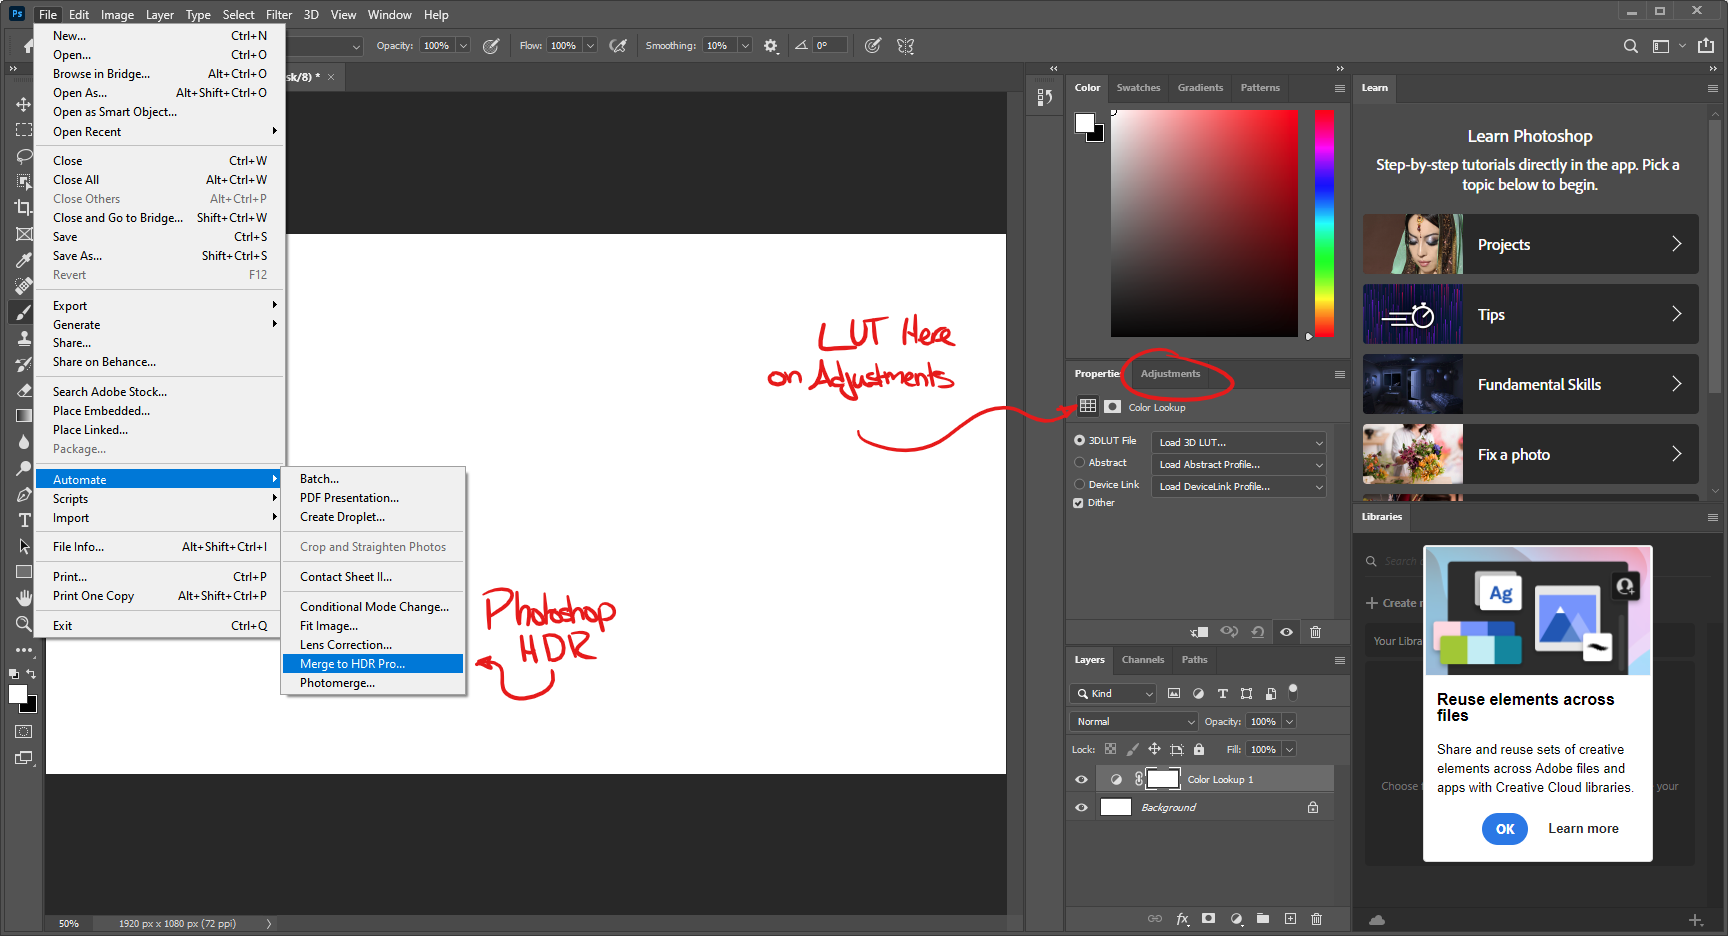
\includegraphics[width=1.0\linewidth]{./img/Photoshop.png}
	\caption{Photoshop HDR and LUT}
	\label{fig:PS-HDR-LUT}
\end{figure}



\end{document}